\documentclass[11pt]{report}
\usepackage{graphicx}
\usepackage{amssymb}
\usepackage{amsthm}
\usepackage{amsmath}
\usepackage{fullpage}
\usepackage{tikz}
\usetikzlibrary{positioning}
\tikzset{node distance=5cm, auto}
\usepackage{cite}
\DeclareGraphicsRule{.tif}{png}{.png}{`convert #1 `dirname #1`/`basename #1 .tif`.png}

\newtheorem{thm}{Theorem}
\newtheorem{prop}{Proposition}
\newtheorem{lemma}{Lemma}
\newtheorem{definition}{Definition}

%%%%%%%%%%%%%%%%%%%%%%%%%%%%%%%%%%%%
%%%%%%%%%%%%%%%%%%%%%%%%%%%%%%%%%%%%
\newcommand{\Q}{\mathbb{Q}}
\newcommand{\Z}{\mathbb{Z}}
\newcommand{\C}{\mathbb{C}}
\newcommand{\R}{\mathbb{R}}
\newcommand{\N}{\mathbb{N}}
\newcommand{\M}{\mathcal{M}}
\newcommand{\Zp}{\mathbb{Z}/p\mathbb{Z}}
\newcommand{\ZP}{\mathbb{Z}/P\mathbb{Z}}
\newcommand{\Zn}{\mathbb{Z}/n\mathbb{Z}}
\newcommand{\Zm}{\mathbb{Z}/m\mathbb{Z}}
\newcommand{\bl}{\ & \ & \\}
\newcommand{\eql}{\ & = &}
\newcommand{\ba}{\\ \begin{array}{rcl}}
\newcommand{\ea}{\end{array} \\}
\newcommand{\claim}{\underline{Claim}: \ }
\newcommand{\pf}{\underline{Proof of Claim}: \\ }
\newcommand{\mat}{\left[\begin{array}{cc} a & b \\ c & d \end{array}\right]}
\newcommand{\lra}{\longrightarrow}
\newcommand{\mf}{\mathfrak}
\newcommand{\inv}{^{-1}}
\newcommand{\ML}{\mathcal{L}}
\newcommand{\LM}{\mathcal{L}}
\newcommand{\LMEF}{\mathcal{L}(E;F)}
\newcommand{\Mnn}{M(n\times n)}
\newcommand{\OnR}{O(n;\R)}
\newcommand{\XM}{\mathfrak{X}(M)}
\newcommand{\eps}{\epsilon}
\newcommand{\CM}{C^{\infty}(M)}
\newcommand{\ddt}{\frac{d}{dt}}
\newcommand{\dds}{\frac{d}{ds}}
\newcommand{\Zhat}{\hat{\mathbb{Z}}}
\newcommand{\coker}{\text{coker}}
\newcommand{\Hom}{\text{Hom}}
\newcommand{\End}{\text{End}}
\newcommand{\Aut}{\text{Aut}}
\newcommand{\Tr}{\text{Tr}}
\newcommand{\ra}{\rightarrow}
\newcommand{\Ra}{\Rightarrow}
\newcommand{\mfp}{\mathfrak{p}}
\newcommand{\mfq}{\mathfrak{q}}
\newcommand{\mfm}{\mathfrak{m}}
\newcommand{\Ap}{A_{\mathfrak{p}}}
\newcommand{\OK}{\mathcal{O}_k}
\newcommand{\Zx}{\mathbb{Z}[x]}
\newcommand{\Zy}{\mathbb{Z}[y]}
\newcommand{\Zxn}{\mathbb{Z}[x_1,\ldots,x_n]}
\newcommand{\Zxy}{\mathbb{Z}[x,y]}
\newcommand{\Zpxy}{\mathbb{Z}/p\mathbb{Z}[x,y]}
\newcommand{\beq}{\begin{equation*}}
\newcommand{\eeq}{\end{equation}}
%\setlength{\parindent}{0cm}        % \noindent everywhere!
%%%%%%%%%%%%%%%%%%%%%%%%%%%%%%%%%%%%
%%%%%%%%%%%%%%%%%%%%%%%%%%%%%%%%%%%%

\setcounter{tocdepth}{2} %show up to subsections in table of contents
\setcounter{chapter}{-1} %first chapter should be 0

\title{Homomorphic Encryption}
\author{Ben LeVeque}
\date{\today}         

\begin{document}
\maketitle


\tableofcontents

\newpage

%%%%%%%%%%%%%%%%%%%%%%%%
%%%%%%%%%%%%%%%%%%%%%%%%
\chapter{Acknowledgements}


%%%%%%%%%%%%%%%%%%%%%%%%
%%%%%%%%%%%%%%%%%%%%%%%%
\chapter{Introduction and background}

\section{Introduction}

In an age of ubiquitous computing, digital security is an important aspect of everyday life. Cryptography is already a pervasive concept, providing privacy for everything from email communication to financial transactions. As computations involving large data sets become more expensive and time-consuming, and as the need for data storage increases, cloud computing has rapidly developed to become a platform to which people and institutions alike turn for their computational needs. With this rise in popularity comes the need for a new class of security protocols that allow data to be stored in encrypted form yet manipulated in a meaningful way by third parties. In this thesis, we consider two such cryptographic schemes. We discuss the motivation behind them, analyze their security, and present data regarding both their security and efficiency. We also provide implementations of the systems in question in C++ and explain the code's design.

Two goals in the very close periphery throughout the development of this project have been reproducibility and accessibility. In this vein, the implementations produced and the data generated are posted in a public repository on Github at https://github.com/bleveque/HomEnc, and a website accompanying the project can be found at (INSERT ADDRESS).

\section{Introduction to cryptographic concepts and terminology} 

Before explaining and analyzing specific schemes, we give a brief background on some common cryptographic concepts. A \emph{cryptosystem} is a collection of procedures that allow a user to securely map a \emph{message} (also called a \emph{plaintext}) $m$ to a \emph{cipertext} $c$ such that the reverse map can only be easily computed given some private information, called a \emph{secret key}. The map taking a message to a ciphertext is referred to as an \emph{encryption function} and in this work will be denoted by $e$, while the reverse map is referred to as a \emph{decryption function} and will be denoted by $d$. The process of determining the secret key is known as \emph{key generation}, and the key generation function will be denoted by $KG$. The messages lie in some space, referred to as the \emph{message space} and sometimes denoted $\M$, and the ciphertexts lie in a (possibly) different space, referred to as the \emph{ciphertext space} and sometimes denoted $\mathcal{C}$, so we have
\begin{align*}
e: \M \lra \mathcal{C} \\
d: \mathcal{C} \lra \M
\end{align*}
A cryptosystem is then given by the collection \[\{\M, \mathcal{C},  KG, e, d\}\] This information together tells us exactly where our messages are coming from and how to encrypt and decrypt them.

\label{Example1}To illustrate the construction above with a brief example, consider the cryptosystem defined by the following elements:
\begin{align*}
&\M = \Z \\
&\mathcal{C} = \Z \\
&KG \text{ gives a random integer } k>1 \\
&e: m \mapsto km \\
&d: c \mapsto c/k
\end{align*}
\noindent This simple scheme encrypts an integer message $m$ by taking its product with the secret key $k$. The resulting ciphertext can be decrypted by dividing by $k$: \[d(e(m)) = d(km) = m\] It is therefore well-defined to encrypt and decrypt a message. This scheme is not very secure, since the value of $k$ can be easily discovered by examining several message/ciphertext pairs, but it is illustrative of the basic ideas.

A lingering question might be ``my message is a regular sentence! how can the message space $\Z$ be of any use to me?'' The answer comes in the form of an invertible \emph{encoding function}. An encoding function is not meant to provide any extra security to our scheme; its sole purpose is to transform real messages into a format we can use in our encryption function. For example, we could encode a word by sending each letter to a number:
\begin{align*}
&a\mapsto 1 \\
&b\mapsto 2 \\
& \vdots \\
&z\mapsto 26
\end{align*}
so the word ``crypto'' would be encoded as the sequence of numbers $\{3,18,25,16,20,15\}$. We could then use our encryption function on each of these numbers. When we decrypt the result, we will get the sequence of numbers back, and then we must perform the inverse of the encoding function to recover our word as a sequence of letters c-r-y-p-t-o.

\

\section{Introduction to homomorphic encryption}
\label{sec:intro_to_hom_enc}

The idea of a homomorphic cryptosystem extends the ideas presented above by adding an additional requirement to the definition. To motivate this requirement, imagine you have a large collection of data points and want to compute their mean or standard deviation. You have have two options: you can either do this computation yourself at a potentially high computational cost, or you can delegate this work to another party and risk losing privacy by exposing your data.  The goal of fully homomorphic encryption is to minimize both potential costs by allowing secure delegation. In practice, this might mean being able to store data on the Cloud in an encrypted form such that a third party could still manipulate the data in a meaningful way. By meaningful, we simply mean that after they operate on our data, we can decrypt the result and obtain exactly the value their operations would have achieved on our original plaintext data. The following diagram illustrates this process:

\

\begin{center}
$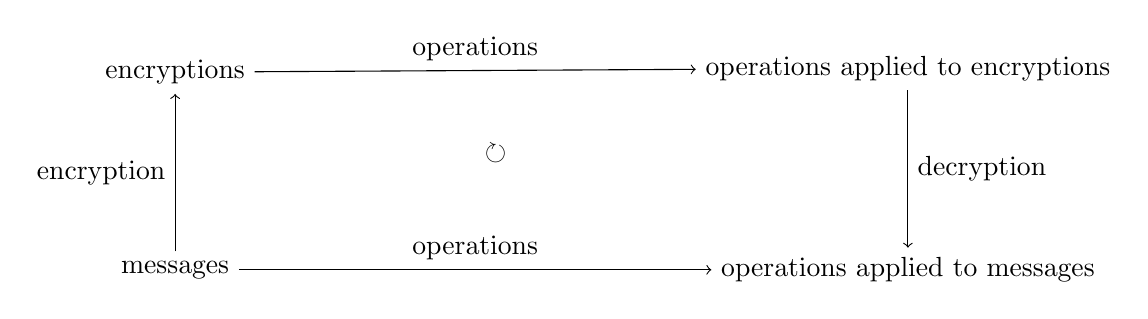
\begin{tikzpicture} \label{hom_diagram}
\node (m) {messages};
\node (fm) [right=6cm of m] {operations applied to messages};
\node (em) [above=2cm of m] {encryptions};
\node (fem) [above=2cm of fm] {operations applied to encryptions};
\node(circarr) [above right=1cm and 3cm of m]{$\circlearrowright$};
\draw[->] (m) to node {operations} (fm);
\draw[->] (fem) to node {decryption} (fm);
\draw[->] (m) to node {encryption} (em);
\draw[->] (em) to node {operations} (fem);
\end{tikzpicture}$
\end{center}

\

Homomorphic encryption ensures that we achieve the same result by traversing this diagram in either direction starting from our messages. More technically, by ``meaningful'' we mean that any combination of sums and products of encryptions decrypt to the corresponding sums and products of the original, unencrypted data. We call such a combination an \emph{arithmetic circuit}, or just a \emph{circuit}. If this were possible, data could be encrypted, operated upon, and decrypted in a completely well-defined manner. What we are looking for, then, is an encryption function that is a \emph{ring homomorphism} from the message space $\M$ to the ciphertext space $\mathcal{C}$. Recall that a ring homomorphism is a map $\sigma: \M \rightarrow \mathcal{C}$ such that for any $x,y\in \M$, \[\sigma(x)+\sigma(y) = \sigma(x+y)\] \[\sigma(x) \sigma(y) = \sigma(xy)\] If our encryption function $e$, then, is a ring homomorphism, we could add or multiply two encryptions and the result would be the encryption of the sum or product of the corresponding plaintexts. A cryptosystem employing such an encryption function is said to give \emph{fully homomorphic encryption} (FHE). If the encryption function in question is a homomorphism in most circumstances, but is not guaranteed to give well-defined decryption after the application of every circuit, the scheme is said to provide \emph{somewhat homomorphic encryption}. Such a scheme might arise if the decryption function requires its input to be of a certain size, which large circuits might exceed. For motivation, consider the following toy example.

\label{Example2}First, we will construct a somewhat homomorphic encryption scheme and then attempt to extend it to be fully homomorphic. Consider the message space $\M = \Z_{\geq 0}$ and choose as a secret key some prime number $p$. We will encrypt a message $m\in \M$ by setting $e(m) = m+ap$ for some random integer $a$. Decryption is then performed by reducing modulo $p$. As long as the message $m$ is less than $p$, this scheme is perfectly well defined, since
\begin{align*}
d(e(m)) &= m+ap \pmod{p}\\
              &= m
\end{align*}
However, if $m\geq p$, then $d(e(m))$ will no longer equal $m$, but will be the reduction of $m$ modulo $p$. One way to attempt to avoid this problem is to encrypt values only less than $p$. However, once we start considering circuits applied to encryptions, this idea shows its flaws; the sum of two encryptions of $p-1$, for example, would really be an encryption of $2p-2$, but it would decrypt to $-2 \equiv p-2 \pmod{p}$. Another solution is to recognize the limitations of the system and include as a part of the system's protocol a bound on the number of additions and multiplications that can be performed on encryptions before the result should be decrypted. 

To make this scheme fully homomorphic, we could set $\M = \Zp$, since in this case, reducing modulo $p$ during decryption is consistent with the structure of the message space. However, it is perhaps unnatural to for messages to live in $\Zp$, since when we compute, for example, standard deviations, we don't want to reduce modulo $p$ at any point during the computation. In this case, it may be best to accept the limitations of the somewhat homomorphic scheme above and work within its framework.

It should be mentioned, as well, that the scheme above is just a ``toy'' example because as in the case of the example on page \pageref{Example1}, it is very insecure. Suppose an eavesdropper asked us to encrypt the message $m=0$ using this system. The result would be a multiple of $p$. Suppose we were asked to perform many such encryptions. We would end up with a collection of multiples of $p$. With this information, it would be very fast to compute the greatest common divisor of these values using the Euclidean Algorithm, and the result would likely be $p$ itself. Using $p$, the eavesdropper could then decrypt any message he pleased by simply reducing it modulo $p$. This type of attack---using encryptions of the message $0$ to reveal an essential feature of the structure of the scheme itself---will appear again, and is a necessary threat to consider when formulating encryption schemes. This attack and others are discussed in the appendix.

%%%%%%%%%%%%%%%%%%%%%%%%%%%
%%%%%%%%%%%%%%%%%%%%%%%%%%%
\chapter{Schemes under investigation}

\section{Introduction to present work}

\
In his 2009 dissertation CITATION, Craig Gentry introduced a fully homomorphic encryption scheme based on the theory of ideal lattices (ideals in polynomial quotient rings). 

\

This thesis will present two encryption schemes and explore their security and efficiency.

In this project, we formulate two schemes that show promise as either somewhat or fully homomorphic encryption schemes. The first,
which is formulated entirely over the integers (and quotient rings thereof), relies on the hardness of making $N$ consecutive correct choices, where each choice
is between two values. We will refer to this as ``choice-based encryption'' (CBE). The second, which is formulated over multivariate polynomial rings, relies on the hardness of the ideal membership problem (IMP) in this
setting. Similar schemes in the past---sometimes referred to as \emph{Polly Cracker} schemes after their introduction by Koblitz and Fellows (CITATION -- from GENTRY AS WELL?)---have been formulated over finite fields. The cryptosystem presented in section~\ref{sec:multicrypt}  below can be formulated over general rings, though we focus on an implementation over the integers. Translating this to an implementation over $\Z/p\Z$ is a matter of reducing coefficients, so while it is easy to reformulate in this setting, the security of the scheme may be compromised, as we will see.

\

\section{Choice-based encryption}

\subsection{Scheme}

We will first describe the scheme in question and subsequently analyze the motivation behind its construction and its cryptographic properties. The choice-based cryptosystem is defined using the following procedures:

\begin{itemize}
\item Key generation ($KG$)
\begin{enumerate}
\item Pick a prime $P$; the message space is $\M := \ZP$
\item Pick a lower bound $M\geq 1$ on the number of operations that our scheme will allow
\item Pick an integer $K$; this is the number of ways we will be able to mask a given message
\item Pick $N\in \Z$ so that $2^N$ is sufficiently large
\item Pick primes $\{p_i\}_{i=1}^N$ such that $((K+1)P)^M<\prod p_i$
\item Pick primes $\{q_i\}_{i=1}^N$
\item Return private key $(N,K,P,\{p_i\},\{q_i\})$ and public key $(N,\{p_iq_i\})$
\end{enumerate}

\item Encryption ($e$)
\begin{enumerate}
\item Pick a message $m\in \M$
\item Pick random integers $\{a_i\}_{i=1}^N$
\item Pick a random integer $k<K$
\item Return $e(m):=(m+kP+a_ip_i \pmod{p_iq_i})_{i=1}^N$; the ciphertext space is $\mathcal{C} := \prod_{i=1}^N(\Z/p_iq_i\Z)$
\end{enumerate}

\item Decryption ($d$)
\begin{enumerate}
\item For all $i=1,\ldots,N$, reduce the $i$th component of the encryption modulo $p_i$
\item Run the Chinese Remainder Theorem with moduli $\{p_i\}$ on the resulting components, which gives $m+kP \pmod{\prod p_i}$
\item Reduce the result modulo $P$ to retrieve $m$
\end{enumerate}

\item Addition of ciphertexts ($+$)
\begin{enumerate}
\item The sum of two ciphertext vectors is their component-wise sum in $\prod (\Z/p_iq_i\Z)$
\end{enumerate}

\item Multiplication of ciphertexts ($\cdot$)
\begin{enumerate}
\item The product of two ciphertext vectors is their component-wise product in $\prod(\Z/p_iq_i\Z)$
\end{enumerate}
\end{itemize}

\subsection{Motivation}

As mentioned above, this scheme is formulated entirely over quotient rings of the integers: the message space is $\ZP$, where $P$ is secret, the ciphertext space is the product of the quotient rings $\Z/p_iq_i\Z$, and the Chinese Remainder Theorem in step two of the decryption function returns a result in $\Z/\prod p_i\Z$. Since we are working strictly with integers (and quotient rings of integers), operations on ciphertexts and messages are easy to describe and implement in code. Simplicity of design is one of the motivations behind the construction, and indeed, it is possible to take $p_i$ and $q_i$ to be quite small as long as our security parameter $N$ is large enough. The underlying hardness assumption is also quite easy to state: given $N$ choices, each between two options, can an eavesdropper identify all $N$ correct options? With a brute-force algorithm, this will take $2^N$ trials, which is computationally infeasible for large $N$. Changing $N$, therefore, affects the hardness of the underlying problem, but increasing its value also increases the size of ciphertexts (by adding components to the encryption vectors). It should be noted, too, that choosing even $N-1$ correct values and a single wrong value for the $\{p_i\}$ (say we choose $q_j$ instead of $p_j$) can give a drastically wrong result, since we would not be completely removing the multiple of $p_j$ in step 1 of decryption, and step 2 of decryption would run the Chinese Remainder Theorem on the wrong collection of primes.

Before proving the correctness and analyzing the characteristics of this system, we will also give some explanation for the other components of the scheme, beginning with the public and private keys. The prime $P$ is the size of our message space. The primes $\{p_i\}$ and $\{q_i\}$ can be chosen arbitrarily as long as the $\{p_i\}$ satisfy the constraints in step 4 of key generation above. The sizes of the primes $p_i$ and $q_i$ are up to the user; larger primes allow for a larger message space, but they also lead to larger ciphertexts. This is a trade-off between efficiency and security that will be analyzed in more depth later on, but for now, we note that it is also possible to create a larger message space by increasing the size of $N$ as well. This will also affect the size of a cipher text, but it has the potential benefit of keeping the values in each component relatively smaller.

The integers $M$ and $K$ together represent the number of ways we can mask or add noise a message with multiples of $P$ before we exceed $\prod p_i$. In other words, we are allowing up to $K$ multiples of $P$ to be added as noise to each component of an encryption, and we are allowing up to $M$ multiplication operations to be performed. We will discuss the implications of these numbers in section~\ref{sec:choice_hom_analysis} below. Note that if we did not allow adding of noise, then it would be easy for an eavesdropper to determine the primes $p_i$ from encryptions of zero. For example, consider a collection of $r$ encryptions of zero (recall that they are not the same, since we choose the values $a_i$ randomly in step 2 of encryption):

\begin{align*}
e(0) &=  (a_{1,1}p_1 \pmod{p_1q_1},\dots,a_{1,N}p_N \pmod{p_Nq_N}) \\
\ &\vdots \ \\
e(0) &= (a_{r,1}p_1 \pmod{p_1q_1},\dots,a_{r,N}p_N \pmod{p_Nq_N})
\end{align*}

\noindent Since reducing an integer $l$ modulo $M$ is done by adding an appropriate multiple of $M$ to $l$, we can express the above as:

\begin{align*}
e(0) &= (a_{1,1}p_1+b_{1,1}p_1q_1,\dots,a_{1,N}p_N + b_{1,N}p_Nq_N) \\
\ &\vdots \\
e(0) &= (a_{r,1}p_1 b{r,1}p_1q_1,\dots,a_{r,N}p_N b_{r,N}p_Nq_N)
\end{align*}

\noindent where the $b_{i,j}$ are the appropriate factors necessary to perform reduction in each component. Now, the $i$th component of each $j$th encryption is a multiple of $p_i$, namely $(a_{j,i}+b_{j,i}q_i)p_i$, so the component-wise GCD of the $r$ encryptions above will likely give us all of the $p_i$, and the security of the scheme (which is based on the difficulty of identifying the $p_i$) will be compromised.

Finally, we note that by setting the message space to $\Z/P\Z$ rather than $\Z$, we ensure that even if a sum or product of messages is greater than $P$, reducing modulo $P$ will give the well-defined sum or product in the message space. In some applications, we may want to ensure that this reduction never occurs (for example, if we are computing statistical quantities over the integers), but it is at least well-defined if it does.

\subsection{Correctness of encryption/decryption}

In order for the choice-based scheme above to be a valid cryptosystem, we need to prove that the composition of encryption with decryption is the identity function on the message space. Formally, we want: \[d\circ e \equiv id_{\ZP}\] We prove this below:

\begin{thm}[Correctness of encryption/decryption for CBE]
If $m\in\ZP$, then $d(e(m)) = m$.
\end{thm}

\begin{proof}
Let $(N,\{p_i\},\{q_i\},K,P)$ be our secret key. Then
\[e(m) = (m+kP+a_ip_i \pmod{p_iq_i})_{i=1}^N\]
for some random $a_i$ and a random $k<K$. Step 1 of decryption performs reduction of each component modulo the corresponding $p_i$, giving
\[\{m+kP \pmod{p_i}\}_{i=1}^N \]
Now, using the Chinese Remainder Theorem in step 2 gives
\[ m+kP \pmod{\prod p_i} \]
Since $m<P$ (here, we are abusing notation slightly and identifying the equivalence class $\bar{m} \in \ZP$ with its minimal representative) and $k<K$, and $P$ was defined such that $(K+1)P <\prod p_i$ (since $M\geq 1$), we have that $m+kP <\prod p_i$, so
\[ m+kP \pmod{\prod p_i} = m+kP\]
Now, reducing modulo $P$ in step 3 gives $m$, since $m\in \ZP$.
\end{proof}


\subsection{Correctness of homomorphic operations}

We now prove that the scheme is somewhat homomorphic up to the desired $M$ multiplications. Note that we measure the level of ``homomorphicity'' using multiplications rather than additions because mulitplications have a larger effect on the size of ciphertexts, and will more quickly cause our numbers to exceed $\prod p_i$. Let us first make the following definitions:

\begin{definition}[Primitive encryption]
A \emph{primitive encryption} $e(m) \in \mathcal{C}$ is an encryption on which no operations have been performed.
\end{definition}

\begin{definition}[$n$-circuit]
An \emph{$n$-circuit} is a sequence of additions and multiplications such that when all multiplications are distributed out, there no more than $n$ total operations in the expression.
\end{definition}

Intuitively, we can think of a primitive encryption as one for which $<K$ multiples of $P$ have been added to each component as noise, as is the case when a message is first encrypted. Now, we will prove correctness:

\begin{thm}[Correctness of homomorphic operations for CBE]
If $C$ is an $M$-circuit which acts on $n\leq M$ values, $C(m_1,\dots,m_n) = d(C(e(m_1),\dots,e(m_n)))$.
\end{thm}

\begin{proof}
Consider two encryptions
\begin{align*}
e(m_1) &= (m_1+ k_1P+a_{1,i}p_i \pmod{p_iq_i})_{i=1}^N\\
e(m_2) &= (m_2+ k_2P+a_{2,i}p_i \pmod{p_iq_i})_{i=1}^N
\end{align*}
Our procedure for addition of ciphertexts tells us that we should perform addition component-wise, so we get
\begin{align*}
e(m_1)+e(m_2) &= (m_1+k_1P+a_{1,i}p_i \pmod{p_iq_i}) + (m_2+ k_2P+a_{2,i}p_i \pmod{p_iq_i}) \\
\ &= (m_1+m_2+ (k_1+k_2)P+(a_{1,i}+a_{2,i})p_i \pmod{p_iq_i})
\end{align*}
Let us assume for the moment that $m_1+m_1+(k_1+k_2)P < \prod p_i$. Then decrypting $e(m_1)+e(m_2)$ gives $m_1+m_2$, so we have that $e(m_1)+e(m_2) = e(m_1+m_2)$ (where equality here really means that $e(m_1)+e(m_2)$ is \emph{an} encryption of $m_1+m_2$, since random numbers are involved in each encryption, so it unlikely that an arbitrary encryption of $m_1$ plus and arbitrary encryption of $m_2$ will equal an arbitrary encryption of $m_1+m_2$). We will return to the question of the size of $m_1+m_2+(k_1+k_2)P$ shortly.

Now consider the product of $e(m_1)$ and $e(m_2)$:
\begin{align*}
e(m_1) e(m_2) &= (m_1+ k_1P+a_{1,i}p_i \pmod{p_iq_i}) \cdot (m_2+ k_2P+a_{2,i}p_i \pmod{p_iq_i}) \\
\ &= (m_1m_2+ (m_1k_2+m_2k_1+k_1k_2P)P+\\
& \ \ \ \ \ \ \ \ \ \ \ ((m_1+k_1P)a_{2,i}+(m_2+k_2P)a_{1,i}+a_{1,i}a_{2,i}p_i)p_i \pmod{p_iq_i})
\end{align*}
In this case, as long as
\[m_1m_2+ (m_1k_2+m_2k_1+k_1k_2P)P < \prod p_i\]
we see that $e(m_1)e(m_2)$ will decrypt as $m_1m_2$ by applying the decryption function. Therefore, $e(m_1)e(m_2)$ is a valid encryption of $m_1m_2$, so $e(m_1)e(m_2) = e(m_1m_2)$. Together with our result for addition, this proves that our scheme is somewhat homomorphic, up to the point that the combination of $m$ and $P$ in each component is less than $\prod p_i$.

We now show that this is the case for any $M$-circuit. Consider the growth of the combination of $m$ and $P$ as we add and multiply encryptions. Primitive encryptions have combinations less than $(K+1)P$, so a sum of two primitive encryptions will have a combination less than $2(K+1)P$ and a product of encryptions will have a combination less than $((K+1)P)^2$. An $M$-circuit with exclusively multiplications will then have a combination less than $((K_1)P)^M$, which by our constraints on the system is less than $\prod p_i$. Since multiplications have a greater effect on the size of the combination than additions, we have shown that our scheme is somewhat homomorphic for all $M$-circuits.

\end{proof}


\subsection{Example of choice-based encryption}
\label{sec:cbe_example}

To illustrate the concepts above, we will carry out a numerical example of encryption, application of circuits, and decryption. For this purpose, we will take our keys to be quite small, letting $N=2$, $M=3$, $K=3$, and $P=7$. Running the key generation function gives us
\begin{align*}
\{p_i\} &= \{263,251\}\\
\{q_i\} &= \{223,263\}
\end{align*}
Note that
\begin{align*}
((K+1)P)^M &= 21952\\
&< 66013\\
&= \prod p_i
\end{align*}
Now, suppose our message is $m=4$. Running the encryption procedure with random values $\{a_i\} = \{11,13\}$ and $k=2$ gives
\begin{align*}
e(4) &= (4+kP+a_1p_1 \pmod{p_1q_1},4+kP+a_2p_2\pmod{p_1q_1}) \\
&= (2911 \pmod{58649}, 3281 \pmod{66013})\\
&= (2911, 3281)
\end{align*}
Now, running our decryption circuit, we first reduce each $i$th component by $p_i$, which gives
\begin{align*}
(2911 \pmod{263}, 3281 \pmod{251}) &= (18,18)
\end{align*}
We next use the Chinese Remainder Theorem, which trivially gives us
\begin{align*}
m+kP &\equiv 18 \pmod{66013}
\end{align*}
Finally, we reduce modulo $P=7$ to get
\begin{align*}
18 &\equiv 4 \pmod{7}
\end{align*}
which matches our original message $m=4$.

Now, we'll give an example of applying a circuit to encryptions. Consider the keys $N=3$, $M=3$, $K=4$, and $P=11$; the messages $m_1=2$, $m_2=4$, $m_3=9$; and the circuit $C(x_1,x_2,x_3) = x_1x_2+x_3$. Since $M=3$, and this circuit has three operations, these operations should be well-defined. Running key generation gives
\begin{align*}
\{p_i\} &= \{97,67,89\}\\
\{q_i\} &= \{107,79,127\}
\end{align*}
Encrypting our three messages (computations omitted for brevity) gives:
\begin{align*}
e(m_1) &= (8097,649,3072)\\
e(m_2) &= (8293,4805,7791)\\
e(m_3) &= (4515,1728,5037) 
\end{align*}
Now, applying our circuit to the encryptions gives
\begin{align*}
C(e(m_1),e(m_2),e(m_3)) &= e(m_1)*e(m_2)+e(m_3)\\
&= (8097\cdot 8293+4515, 649\cdot 4805+1728, 3072\cdot 7791+5037)\\
&= (806,2596,10538)\\
\end{align*}
Decrypting this gives
\begin{align*}
d(C(e(m_1),e(m_2),e(m_3))) &= 6
\end{align*}
Applying our circuit to our unencrypted messages likewise gives
\begin{align*}
C(m_1,m_2,m_3) &= m_1m_2+m_3\\
&= 6
\end{align*}
(recall that our messages are elements of $\ZP$). This shows that the diagram on page~\pageref{hom_diagram} is indeed commutative for our example. 



\subsection{Analysis of homomorphicity in practice}
\label{sec:choice_hom_analysis}

In practice, we may want to know the most efficient way to increase the number of homomorphic operations supported by our system. Since the parameters of the scheme tell us that
\begin{align*}
\#ops &\geq \log_{(K+1)P}\left(\prod_{i=1}^N p_i\right)
\end{align*}
we have several options for parameters to alter. We can decrease $K$, decrease $P$, increase $N$, or increase the values of the $p_i$. Decreasing $P$ or $K$ affects the security of the system, since we would have either a smaller message space or fewer ways to mask encryptions. On the other hand, increasing the size of each prime $p_i$ will increase the size of the ring $\Z/p_iq_i\Z$ in each component of an encryption, and will therefore cause our arithmetic on encryptions to run more slowly. Increasing $N$ (and maintaining the size of the $p_i$ and $q_i$) has a similar effect; now we have more components in each encryption, so arithmetic will be less efficient. However, increasing $N$ has the added benefit of increasing the complexity of a brute-force search through all $2^N$ combinations of $p_i$ and $q_i$.

Which option should we take in practice? In increasing the number of operations allowed, we certainly do not want to negatively impact the security or flexibility of our scheme, so decreasing $K$ or $P$ is not ideal. It would seem, then, that increasing $N$ might be provide the greatest benefit: increasing the number of multiplications (by increasing the product $\prod p_i$) while also increasing the complexity of brute-force search. Analyzing this problem further would be an interesting application of the implementations outlined in chapter~\ref{chap:implementation}.

\

An additional concern is that our message space may not realistically resemble $\Zp$, for example if the information we want to encode is a collection of integer values, and we want to compute the product of these integers, we expect the result of performing the encrypted operation to be the true product, even if it exceeds $P$. As soon as the results of computations exceed $P$, the scheme fails to return the correct value to the user, so practically speaking, we want our messages to be much smaller than $P$, which is in turn much smaller than $\prod p_i$. Precisely, this means that requiring that any message $m$ satisfy $m<\sqrt[M]{P}$ guarantees that products of messages will always decrypt properly, since $M$ is the number of allowed multiplications from above. In practice, this means that if we want our operations to remain in the integers, we should set $\M = \Z_{<\sqrt[M]{P}}$.

\

A desirable aspect of any cryptosystem is that the size of any ciphertext is not excessively large relative to the size of its corresponding plaintext. In this system, including the considerations in the paragraph above, a message $m$ has worst-case size $|m|=\sqrt[M]{P}$, while a ciphertext has size
\begin{align*}
\sum_{i=1}^N\left|(\Z/p_iq_i\Z)\right| &= \sum_{i=1}^Np_iq_i
\end{align*}
Note that if we did not reduce each component modulo $p_iq_i$, our ciphertexts could grow quite rapidly. Also, since we're reducing modulo $p_iq_i$, we do not experience any ciphertext expansion when we apply circuits to ciphertexts. [[[[[According to (CITATION OF P.C.R), this scheme is called \emph{compact}, meaning that there is a fixed polynomial bound on the size of ]]]]]


\subsection{Security}
\label{sec:cbd_security}



\section{Using multivariate polynomial rings}
\label{sec:multicrypt}

Another approach to homomorphic encryption is to use the properties of arithmetic in polynomial rings. The ring structure essentially guarantees that if our encryption involves only arithmetic operations, it will be homomorphic. Perhaps the most natural thing to try in this setting is the following algorithm: choose a principal ideal $(f)\subset \Zx$ and encrypt an integer message $m$ by adding a random element $af\in (f)$, so $e(m) = m+af$. Then to decrypt, we simply reduce modulo the polynomial $f$. This process is homomorphic because ideals are closed under addition and multiplication:
\[e(m_1)+e(m_2) = m_1+m_2+(a_1+a_2)f= e(m_1+m_2)\]
and
\[e(m_1)e(m_2) = m_1m_2+(m_2a_1+m_1a_2+a_1a_2)f = e(m_1m_2)\]
Note that our definition of equality above is somewhat loose; since $e(m_1+m_2)$ encrypts by choosing a \emph{random} multiple of $f$, it may not be exactly $(a_1+a_2)f$ (and likewise for the case of multiplication). The notion of equality we adopt, then, is a notion of coset equality: $e(m_1)+e(m_2)$ is in the same coset of $I$ as $e(m_1+m_2)$, so they will decrypt identically, and the same is true for $e(m_1)e(m_2)$ and $e(m_1m_2)$.

While this scheme illustrates the ideas we will use later, it is not very secure on its own. For example, suppose an eavesdropper, Eve, asks us to encrypt $m=0$ several times. The resulting ciphertexts would be a collection
\[\left\{ a_1f_1, a_2f_2,\dots ,a_nf_n\right\}\]
Now, if Eve takes the greatest common divisor of the elements in this collection (note that this is very similar attack employed to break the toy example in section~\ref{sec:intro_to_hom_enc}), there is a very high chance that the result will be $f$ itself or a small multiple of $f$. With $f$ in hand, Eve could then decrypt any message she pleased, and the scheme would be compromised.

The scheme above was easily broken because it relied on a fairly easy problem: given a collection of polynomials in a principal ideal, find a generator for the ideal. This is easily found because we can compute fairly efficiently the greatest common divisor of two polynomials in $\Z[x]$. This is a basic case of a more general problem:

\begin{definition}[Ideal Membership Problem (IMP)]
Given a ring $R$, a set of elements $\{r_1,\dots,r_n\}\in R$, and an element $f\in R$, determine whether $f\in (r_1,\dots,r_n) \subset R$.
\end{definition}

If the structure of $R$ is simple, then this problem is correspondingly easy, as we saw above in the case of our set of generators being multiples of a single polynomial $f\in \Zx$. The ease of solution here comes from the fact that greatest common divisors are fairly easy to compute over $\Zx$; with the greatest common divisor of our generators available, we can easily reduce further encryptions by the common divisor to reveal their corresponding plaintexts. However, if we look instead at multivariate polynomial rings such as $\Zxy$ or $\Zpxy$, the problem might not be so simple. GIVE EXAMPLE OF THE NECESSITY OF ORDERING MONOMIALS. It is with this motivation that we formulate the following scheme:

\

\subsection{Scheme}

The scheme goes as follows:

\begin{itemize}
\item Key generation ($KG$)
\begin{enumerate}
\item Set $\M := \Z$ and $\mathcal{C} := \Zxy$
\item Pick a degree bound $D$ and a coefficient bound $B$
\item Pick a random number $z_0 < B$
\item Pick a random polynomial $f$ with total degree less than or equal to $D$ and coefficients less than $B$
\item Pick a random polynomial $g'$ of total degree less than or equal to $D-1$ and coefficients less than $B$
\item Set $g := (y-z_0)g'$
\item Return private key $(f,g,z_0)$
\end{enumerate}

\item Encryption ($e$)
\begin{enumerate}
\item Pick a message $m\in \Z$
\item Pick random polynomials $a$ and $b$ which respect the degree and coefficient bounds
\item Return $e(m) := m+af+bg$
\end{enumerate}

\item Decryption ($d$)
\begin{enumerate}
\item Evaluate the encryption at $z_0$
\item Reduce the result modulo $f(x,z_0)$, a single-variable polynomial, and return the result
\end{enumerate}

\item Addition of ciphertexts ($+$)
\begin{enumerate}
\item Given two ciphertexts in $\Zxy$, their sum is simply their sum as multivariate polynomials
\end{enumerate}

\item Multiplication of ciphertexts ($\cdot$)
\begin{enumerate}
\item Given two ciphertexts in $\Zxy$, their product is simply their product as multivariate polynomials
\end{enumerate}
\end{itemize}

\subsection{Explanation}
Before analyzing the security properties of this scheme, we give a brief summary of its procedures. Key generation uses degree and coefficient bounds to create a secret root $z_0$ and secret polynomials $f$ and $g$, where $g$ vanishes on the line $y=z_0$. The fact that $g$ vanishes at $(x,z_0)$ for all $x\in \Z$ allows us to evaluate an encryption at $(x,z_0)$ to eliminate the $bg$ term completely. We are then in a single-variable setting (evaluating at $(x,z_0)$ is essentially a map $\Zxy \ra \Zx$), and can then easily reduce modulo $f(x,z_0)$. It is then easy to encrypt and decrypt, since we are only performing simple polynomial arithmetic, evaluating polynomials, and reducing modulo one-variable polynomials. We prove below that this gives a well-defined encryption scheme. We note also that the degree and coefficient bounds can be chosen as to make the underlying hard problem (discussed in section~\ref{sec:mv_security} below) difficult. In chapter~\ref{chap:implementation}, we discuss the problem of choosing appropriate bounds.

One benefit of using polynomials for encryption, as we will prove below, is that since our message is zero-degree (i.e. an integer), there is no limit on the number of additions and multiplications we can perform.


\subsection{Correctness of encryption/decryption}
We will now prove the well-definition of encryption and decryption using 


\begin{thm}[Correctness of encryption/decryption for multivariate encryption] If $m\in \Z$, then $d(e(m)) = m$.
\end{thm}

\begin{proof}
First, encryption gives us
\[e(m) = m+af+bg\]
for some $a$ and $b$, where we know that $g(x,z_0)=0$ by construction. In step 1 of decryption, we evaluate at $(x,z_0)$, giving
\[e(m)(x,z_0) = m+a(x,z_0)f(x,z_0)\]
This is a single variable polynomial which can be reduced modulo the polynomial $f(x,z_0)$ (this is known to the decryptor, since $f$ and $z_0$ are both components of the secret key) to give $m$, since $m$ is simply a constant value and will not be affected by reduction by any non-constant polynomial. This proves correctness.
\end{proof}


\subsection{Correctness of homomorphic operations}

Now we prove that sums and products of encryptions are valid encryptions of the sums and products of the corresponding plaintexts. Unlike the choice-based scheme, there is no limit on the number of operations that can be performed on ciphertexts (i.e. we can apply an $n$-circuit for any $n$ in a well-defined manner).

\begin{thm}[Correctness of homomorphic operations for multivariate encryption] If $m_1,m_2 \in \Z$, then $e(m_1)+e(m_2) = e(m_1+m_2)$ and $e(m_1)e(m_2) = e(m_1m_2)$.
\end{thm}

\begin{proof}
Note first that two ciphertexts are encryptions of the same value if and only if they lie in the same coset of $(f,g)\subset \Zxy$. The encryptions $e(m_1)$ and $e(m_2)$ are of the form
\begin{align*}
e(m_1) &= m_1+a_1f+b_1g\\
e(m_2) &= m_2+a_2f+b_2g
\end{align*}
for some $a_i,b_i\in \Zxy$. Then
\begin{align*}
e(m_1)+e(m_2) &= m_1+m_2 +(a_1+a_2)f+(b_1+b_2)g
\end{align*}
This is in the coset $m_1+m_2$ of $(f,g)$, so it is indeed an encryption of $m_1+m_2$. This proves that the scheme is additively homomorphic. Consider the product now:
\begin{align*}
e(m_1)e(m_2) &= m_1m_2+(m_1a_2+m_2a_1)f+((m_1+a_1f)b_2+(m_2+a_2f)b_1)g
\end{align*}
This is in the coset $m_1m_2$ of $(f,g)$, so it is an encryption of $m_1m_2$. This proves that the scheme is multiplicatively homomorphic as well.
\end{proof}
At no point in the proof above does the size of either message affect the ability of the scheme to encrypt and decrypt properly; the scheme is fully homomorphic in the sense that arbitrary-depth circuits can by applied homomorphically.


\subsection{Example of multivariate encryption}
\label{sec:mv_example}
We will now work out an example using the multivariate encryption scheme above. Let us choose $D=2$ and $B=10$. Running the key generation step, we get
\begin{align*}
z_0 &= 6\\
f &= 4xy+6y+1\\
g &= y^2+3y-54
\end{align*}
Note that it is coincidence only that $g$ is a polynomial in $\Zy$. Also, its constant coefficient is larger than our coefficient bound! The reason for this transgression is that $g$ is generated as a product of a random polynomial (which does adhere to the degree bound) and the polynomial $(y-z_0)$, so $g$ itself may have coefficients as large as $B^2$.

Now, suppose we want to encrypt $m=1024$. Running our encryption procedure with random polynomials
\begin{align*}
a &= 5xy+x+y+5\\
b &= 3xy+8x+3y+1
\end{align*}
we get
\begin{align*}
e(m) &= m+af+bg\\
&= 20x^2y^2 + 3xy^3 + 4x^2y + 75xy^2 + 3y^3 - 107xy + 52y^2 - 431x - 122y + 975
\end{align*}
Now, we run our decryption circuit by first plugging in $z_0=6$, which gives
\begin{align*}
e(m)(x,z_0) &= 20x^2(6^2) + 3x(6^3) + 4x^2(6) + 75x(6^2) + 3(6^3) - 107x(6) + 52(6^2) - 431x - 122(6) + 975\\
&= 744x^2 + 2275x + 2763
\end{align*}
Finally, we reduce modulo $f(x,z_0)$ to get
\begin{align*}
e(m)(x,z_0)\pmod{f(x,z_0)} &= (744x^2 + 2275x + 2763) \pmod{24x + 37} \\
&=1024
\end{align*}
This is indeed our original message, which shows that encryption/decryption is well-defined for this example.

We now give an example of a circuit applied to three encryptions (in fact, the same circuit as we used in section~\ref{sec:cbe_example}), namely $C(x_1,x_2,x_3)=x_1x_2+x_3$. Suppose we want to encrypt $m_1=123$, $m_2=234$, and $m_3=345$ and apply the circuit $C$ to the encryptions. We show this process below (omitting some computations for brevity). First, running key generation gives
\begin{align*}
f &= 7xy+5x+6y+5\\
g &= 2xy-14x+3y-21\\
z0 &= 7
\end{align*}
Now, encrypting our messages gives:
\begin{align*}
e(m_1) &= 42x^2y^2-42x^2y-36x^2+45xy^2-42xy-137x+51y+1\\
e(m_2) &= 24x^2y^2-60x^2y+34xy^2- 44xy+2x+6y^2+47y+222\\
e(m_3) &= 42x^2y^2-15x^2y+45x^2+62xy^2-78xy+57x+21y^2-46y+343\\
\end{align*}
Applying the circuit $C$ to these encryptions gives
\begin{align*}
C(e(m_1),e(m_2),e(m_3)) &= e(m_1)e(m_2)+e(m_3)\\
&= 1008x^4y^4-3528x^4y^3+1656x^4y^2+2160x^4y+2508x^3y^4-6984x^3y^3-\\
& \ \ \ \ \ \ 60x^3y^2+9720x^3y-72x^3+1782x^2y^4-462x^2y^3+1420x^2y^2-\\
& \ \ \ \ \ \ 5147x^2y-8221x^2+270xy^4+3597xy^3+5046xy^2-15783xy-\\
& \ \ \ \ \ \ 30355x+306y^3+2424y^2+11323y+565
\end{align*}
As a brief aside, note that in this scheme, ciphertexts grow quite quickly as we apply circuits. We will discuss this in more depth in section~\ref{sec:mv_hom_analysis} below. Now, decrypting the result above gives
\begin{align*}
d(C(e(m_1),e(m_2),e(m_3))) &= C(e(m_1),e(m_2),e(m_3))(x,z_0) \pmod{f(x,z_0)}\\
&= 29127
\end{align*}
Now, applying $C$ to the original messages gives
\begin{align*}
C(m_1,m_2,m_3) &= m_1m_2+m_3\\
&= 29127
\end{align*}
This shows that applying a circuit is well-defined for this example.

\subsection{Practical analysis of homomorphicity}
\label{sec:mv_hom_analysis}
Unlike the choice-based scheme above, this scheme as presented suffers from significant ciphertext expansion as circuits with a large number of multiplications are applied. Sums of ciphertexts do not grow in size too quickly, because when two ciphertexts are added, the degree of the result will not have grown. The coefficients roughly double in an addition, but this is negligible when compared to the result of a multiplication. When two ciphertexts (of comparable degree) are multiplied, the total degree of the result is roughly twice the total degree of the initial ciphertexts. Let $d$ be the maximum of the maximum $x$-degree and $y$-degree of the product. Since we are working with two variables, there are roughly $d^2$ possible terms, each having coefficients larger than those in the initial ciphertexts. For example, the coefficient of the highest degree term will be the product of the corresponding highest-degree coefficients of the original ciphertexts, and the coefficients of smaller degree terms will be sums of such products, leading to very fast coefficient growth.

There are then two issues with homomorphic operations in this scheme: coefficient growth and degree growth. In order to combat coefficient growth, we could imagine setting up our scheme with $\mathcal{C} = \Zpxy$ for some prime $p$ rather than $\mathcal{C} = \Zxy$. We will discuss the feasibility of this possibility in more depth in section~\ref{sec:mv_security} below. To attempt to deal with degree growth, we could consider making an encryption of $m=0$ public knowledge. In particular, we could choose one encryption of zero which lies entirely in $\Zx$ and one which lies entirely in $\Zy$. FINISH


\subsection{Security}
\label{sec:mv_security}
We now look at the security characteristics of this system. We have seen that the scheme is constructed to rely on the hardness of the Ideal Membership Problem for multivariate polynomial rings. In particular, encryptions of $m=0$ lie in $(f,g)\subset \Zxy$, so if there is a procedure to efficiently decide whether an element of $\Zxy$ is in the ideal $(f,g)$, we would be able to test whether arbitrary encryptions are encryptions of $0$. The ability to do so would be disastrous for the the security of our system; beyond simply being able to test if we are sending the message $m=0$ (which we could always avoid doing if need be), it allows us to \emph{compare} encryptions. We know that any two encryptions of a message $m\in \M$ are in the same coset of $(f,g)$, so their difference will be in the coset of $0$ (namely, it will be in $(f,g)$). Therefore, if an eavesdropper collects several plaintext/ciphertext pairs, she essentially has a table of encryptions to check any future encryptions against. For example, if our message space is small, an eavesdropper could perform a lunchtime (CITATION) attack and ask our encryption scheme to encrypt each of the possible messages, and then when she intercepts any message, she could easily determine its value based on her knowledge and ability to recognize encryptions of zero.

The tool that helps solve the IMP in polynomial rings is called a \emph{Gr\"obner basis}.


\subsection{Generalizing}

... One benefit to this scheme is that it can be easily generalized to $n$ variables -- i.e. we can consider an analogous scheme over $\Zxn$. This is done by choosing $g$ such that $g(x_1,\ldots,x_n) = g_1(x_1)g_2(x_2)\cdots g_n(x_n)$ and $z_2,\ldots,z_n$ such that $z_i$ is a root of $g_i$. Then encryption proceeds as in the two-variable case:

$\ba
e(m) & = & m + af + bg
\ea$

and to decrypt, we first evaluate at $(x_1,z_2,\ldots,z_n)$ and then reduce modulo $f(x_1,z_2,\ldots,z_n) \in \Z[x_1]$. Further tests would be necessary to see if increasing the number of variables is an effective way to increase the computational complexity of Groebner basis computation. 

\


\chapter{Applications}

Beyond theoretical formulation, it is important to see how these schemes might perform in practice. As mentioned in the introduction, the efficiency of homomorphic schemes has been a major obstacle to their dissemination, and 

\section{Application to medical needs}

\

\section{Application to finance}

\ EXAMPLE OF STD-DEV

A significant drawback of using our choice-based encryption scheme for the manipulation of statistics is made apparent when we consider taking the standard deviation of many numbers. This requires being able to make a large number of well-defined multiplications, which may be impossible, especially if the numbers in question are large. Problems like this may be more suited to our multivariate scheme, which can make arbitrary numbers of well-defined multiplications. We may lose efficiency, but in computations that require correctness over

\chapter{Implementation}
\label{chap:implementation}

\

\chapter{Appendix}

\section{Common notation and terminology}

We recall in this section some commonly used notation used throughout the preceding pages:

\begin{itemize}
\item $\Z$ --- the ring of integers, i.e. $\{\dots,  -2, -1, 0, 1, 2, \dots\}$
\item $\Zp$ --- the ring of integers modulo $p$, i.e. the set of equivalence classes $\{\bar{0}, \bar{1}, \dots , \bar{(p-1)}\}$
\item $R[x_1, \dots ,x_n]$ --- the ring of polynomials in the variables $x_1,\dots, x_n$ with coefficients in the ring $R$; used most often above is the ring of polynomials with integer coefficients, $\Z[x_1,\dots,x_n]$
\item A \emph{commutative diagram} is a visual representation of a collection of maps which can be applied in multiple ways to get the same result. For example, if we have the maps 
\begin{align*}
f: & \ \R^2 \lra \R\\
&(x,y)\mapsto x+y\\
\\
g : & \ \R^2 \lra \R^2\\
&(x,y)\mapsto (2x,2y)\\
\\
h : & \ \R^2\lra \R^2\\
&(x,y)\mapsto (\frac{x}{2},\frac{y}{2})
\end{align*}
the following commutative diagram represents the fact that adding two numbers is the same as first multiplying both by $2$, adding them, and then dividing the product by $2$:


\begin{center}
$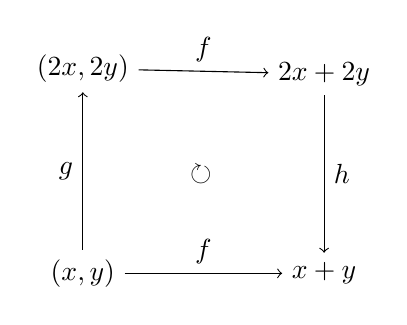
\begin{tikzpicture} \label{comm_diagram_ex}
\node (m) {$(x,y)$};
\node (fm) [right=2cm of m] {$x+y$};
\node (em) [above=2cm of m] {$(2x,2y)$};
\node (fem) [above=2cm of fm] {$2x+2y$};
\node(circarr) [above right=1cm of m]{$\circlearrowright$};
\draw[->] (m) to node {$f$} (fm);
\draw[->] (fem) to node {$h$} (fm);
\draw[->] (m) to node {$g$} (em);
\draw[->] (em) to node {$f$} (fem);
\end{tikzpicture}$
\end{center}


\end{itemize}

\section{Common Attacks}

This section is a compilation of and reference for some of the types of attacks considered in the duration of this project.

\begin{itemize}
\item gcd attacks
\item G.B. attacks (type of gcd)
\item using known encryptions of zero to identify encryptions of the same value
\item
\end{itemize}

\

\section{An intro to Gr\"obner bases}

\

\section{Failed Attempts}

\section{Notes}
Cite Donald Knuth, Art of Computer Programming, Addison-Wesley Publishing Company, Reading, Massachusetts, second addition, pp 273-4 for representation of multivariate polynomials using linked lists.

\

Cite Gentry, Fellows and Koblitz

\

Page 38 of HPS

\

Changed RAND to RAND2 after a bunch of tests already computed. Initially, we were using just products of random numbers to generate new random numbers, but there was an issue that if any of these random numbers were even, all subsequent ones would be as well, implying that most coefficients were probably even (since the bounds we use are powers of two). It is changed to increase by multiplying by a rand and also adding one. Also changed it to make constant coefficients non-zero, since constant coeffs help to hide the message. Also changed the coeffs of random polys to between coeffbd and 1 rather than coeffbd and coeffbd/2.

\

32749 is the largest prime usable in M2 for polynomial rings over finite fields

\

Note that coeffsize doesn't matter so much for Z/pZ, since arithmetic is all Z/pZ

\

Cite sage, M2, singular, c++, GMP, d3

\

Idea: get f.resultant(g,x) and f.resultant(g,y) to reduce encryptions by!

\end{document}  